\section{Què és?}

La intel·ligència artificial és aquella branca de la informàtica dedicada al
desenvolupament d'algorismes per aconseguir que una màquina prengui decissions
 racionals per si mateixa o que es comporti de forma similar a la intel·ligència humana.

Resumint, segons la definició més estesa, que és la de l'informàtic i
investigador cognitiu estadounidenc \emph{John McCarthy}, és \emph{"Fer que una màquina
es comporti d'una manera que en un humà considerariem intel·ligent"}.

En el que a robòtica es refereix la intel·ligència artificial consisteix a aplicar la
definició anterior, és a dir, un ésser no viu amb una intel·ligència racional semblant
a la humana, a una estructura que sol tenir una fisiologia semblant a la nostre i que
es pot moure.
\cite{definiciondeia} \cite{wikiia} \cite{monoia}

\section{Principals utilitats}

És interessant veure a on s'utilitzen mètodes d'IA en l'actualitat. És també complicat fer-ho sense reflexionar una mica, ja que la convicció popular de IA és relacionada amb la simulació del caràcter humà, i si més no estem encara una mica lluny d'aquest objectiu, hi ha una gran quantitat d'aplicacions que utilitzen petits procediments de forma similar a com ho faria un humà.

La IA s'utilitza diàriament en àmbits extremadament diversos: diagnosi mèdica \ref{diagnosis}, comerç amb stock, control de robots, llei, traducció de textos \ref{translate}, domòtica, visió artificial \ref{cat}, etc.


\begin{figure}[ht!]
\centering
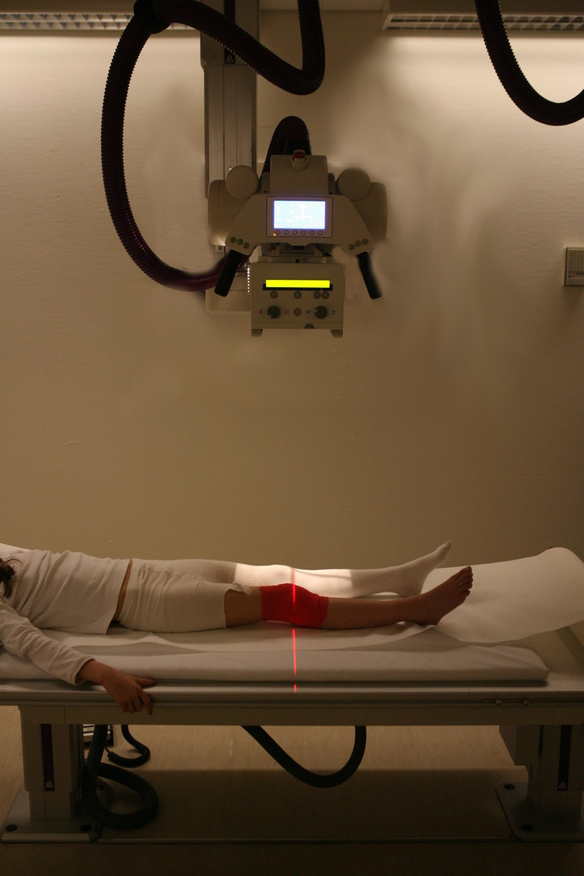
\includegraphics[height=60mm]{data/diagnosis_2.jpg}
\caption{S'estan dissenyant sistemes de \emph{diagnosi mèdica}, que seran entrenats per a, per exemple, distingir teixits cancerígens en imatges.}
\label{diagnosis}

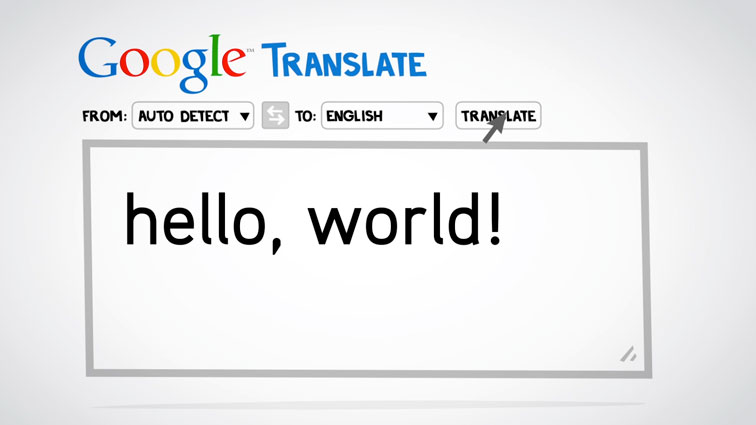
\includegraphics[width=60mm]{data/translate.jpg}
\caption{S'utilitza de forma diària, però molts pocs saben que darrere d'una interfície d'usuari senzilla s'amaga un sistema de traducció intel·ligent molt diferent a la traducció literal paraula per paraula.}
\label{translate}

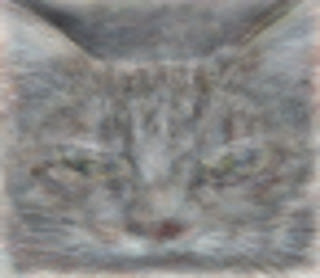
\includegraphics[width=75mm]{data/cat.jpeg}
\caption{Desenvolupadors de Google han entrenat una \emph{xarxa neuronal} per a que identifiqui cares de gats en vídeos a YouTube. Aquesta es la visió generalitzada d'un gat, després de milers de vídeos d'entrenament. \cite{googlecat}}
\label{cat}
\end{figure}
